\documentclass{article}
\usepackage[utf8]{inputenc}
\usepackage{hyperref}
\usepackage[letterpaper, portrait, margin=1in]{geometry}
\usepackage{enumitem}
\usepackage{amsmath}
\usepackage{booktabs}
\usepackage{graphicx}
\usepackage{mathtools}  
\usepackage{diffcoeff} 
\usepackage{hyperref}
\usepackage{physics}
\hypersetup{
colorlinks=true,
    linkcolor=black,
    filecolor=black,      
    urlcolor=blue,
    citecolor=black,
}
\usepackage{natbib}

\usepackage{titlesec}
\usepackage{chngcntr}

\counterwithin*{equation}{section}
\counterwithin*{equation}{subsection}


  
\title{Homework 6}
\author{Economics 7103}
\date{Spring semester 2023}
  
\begin{document}

\maketitle
\section{Python}
\subsection{}
This should be a sharp RD as all cars longer than 225 inches are treated, impacting their MPG. However, outliers may exist. 
\newline

\subsection{}
\begin{figure}[ht]
    \centering
    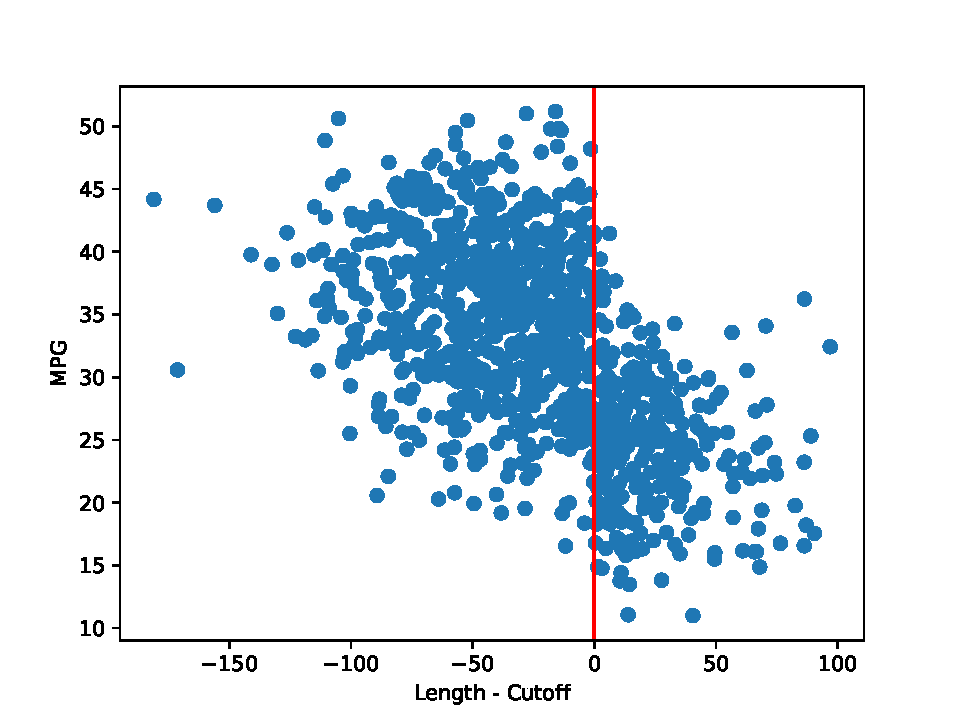
\includegraphics{Q2-1.pdf}
    \caption{MPG vs Length}
    \label{fig:my_label}
\end{figure}

Bunching is defined as the pattern where data points seem to cluster in specific regions. There does not seem to be any evidence of bunching (Figure 1). However, there does seem to be a discontinuity at the cutoff for MPG.   
\newline

\subsection{}

The treatment effect is -8.27 mpg for the treated as shown in Table 1. The figure associated with it is Figure 2. 
\begin{table}[!htbp] 
\caption{First order polynomial RD}
\centering
\begin{tabular}{@{\extracolsep{5pt}}lc}
\\[-1.8ex]\hline
\hline \\[-1.8ex]
& \multicolumn{1}{c}{\textit{Dependent variable:}} \
\cr \cline{1-2}
\\[-1.8ex] & (1) \\
\hline \\[-1.8ex]
 Treated & -8.27$^{***}$ \\
  & (0.65) \\
 Length minus Cutoff & -0.04$^{***}$ \\
  & (0.01) \\
 Constant & 33.76$^{***}$ \\
  & (0.41) \\
\hline \\[-1.8ex]
 Observations & 1,000 \\
 $R^2$ & 0.40 \\
 Adjusted $R^2$ & 0.40 \\
 Residual Std. Error & 6.16  \\
 F Statistic & 389.15$^{***}$  \\
\hline
\hline \\[-1.8ex]
\textit{Note:} & \multicolumn{1}{r}{$^{*}$p$<$0.1; $^{**}$p$<$0.05; $^{***}$p$<$0.01} \\
\end{tabular}
\end{table}
\begin{figure}[ht]
    \centering
    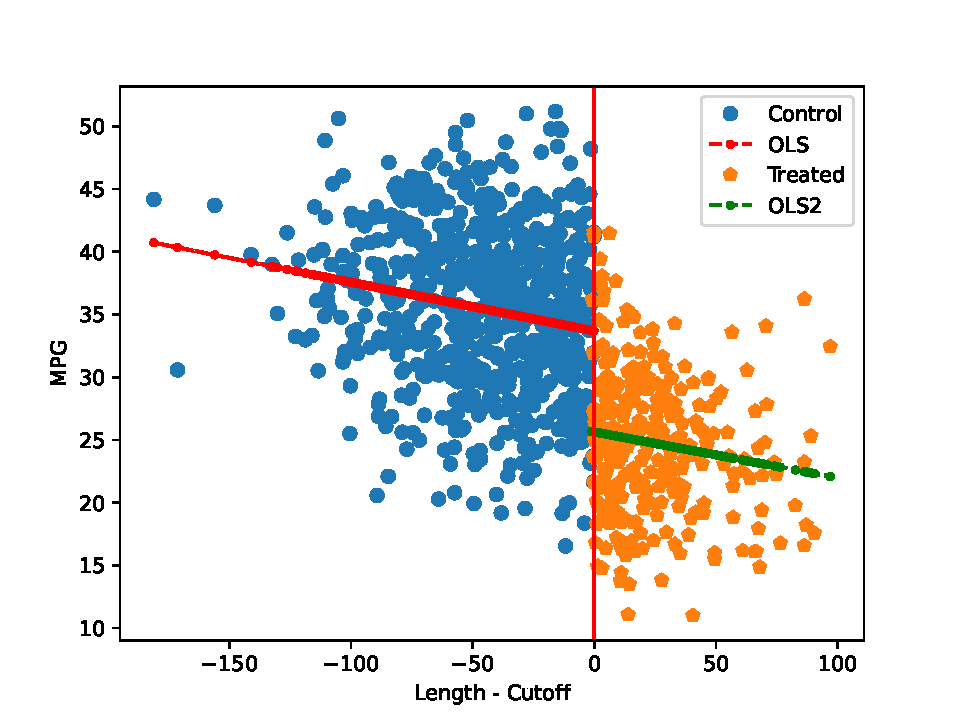
\includegraphics{Q3-1.pdf}
    \caption{First order polynomial fit}
    \label{Figure2: FO}
\end{figure}


\subsection{}
The first stage treatment effect is 0.0002. RD plot: Fig3.
\begin{figure}[ht]
    \centering
    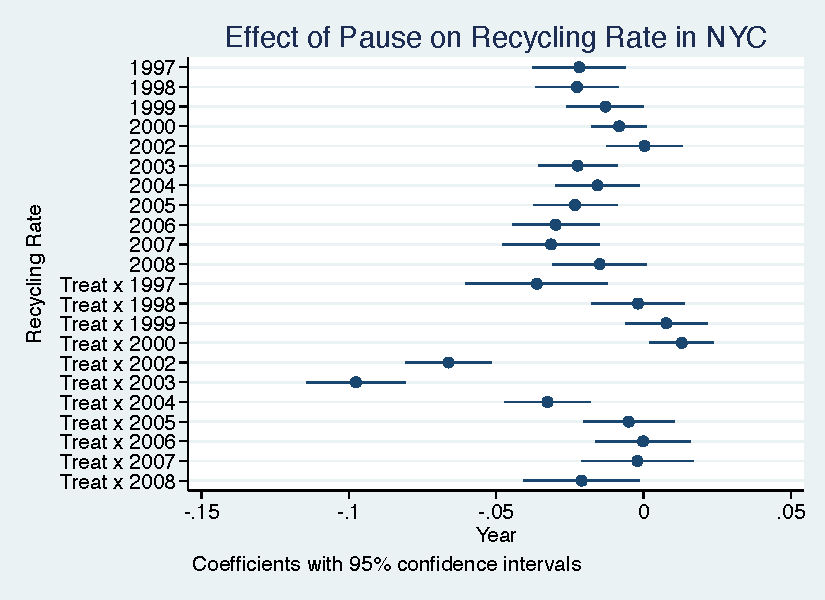
\includegraphics{Q4.pdf}
    \caption{Second order polynomial fit}
    \label{fig:my_label}
\end{figure}

\subsection{}
The treatment effect is 1.525. RD plot: Fig4. 
\begin{figure}[ht]
    \centering
    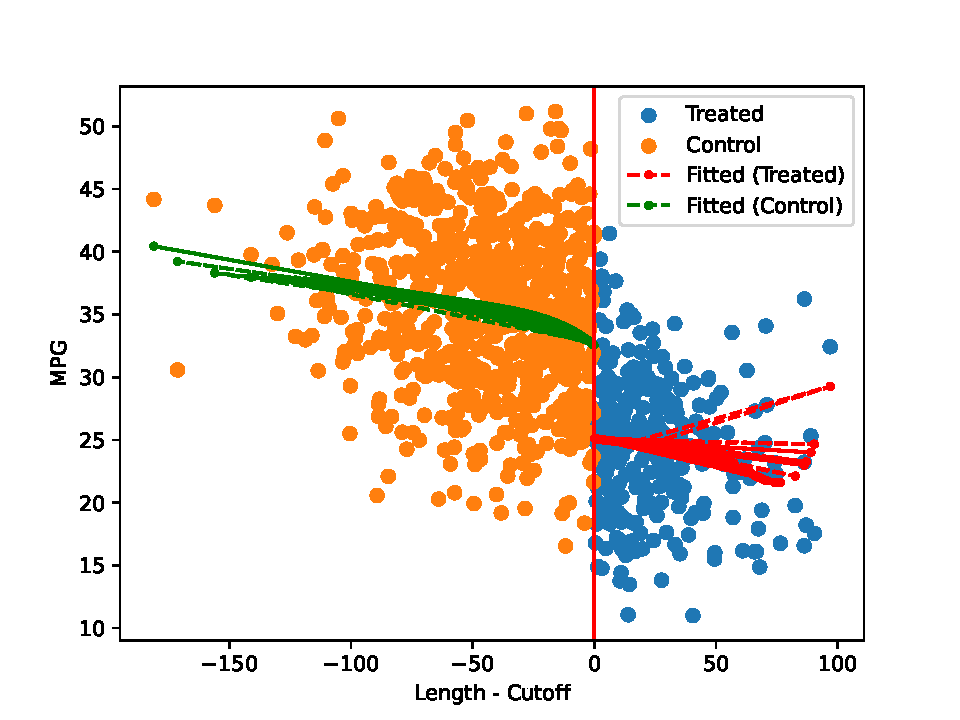
\includegraphics{Q5.pdf}
    \caption{Fifth order polynomial fit}
    \label{fig:my_label}
\end{figure}

\subsection{}
The average treatment effect is -735.62. 

\section{Stata}

\subsection{}
Summary stats: Table 2
\begin{table}[ht]
    \centering
    \documentclass[]{article}
\setlength{\pdfpagewidth}{8.5in} \setlength{\pdfpageheight}{11in}
\begin{document}
\begin{tabular}{lc}
\multicolumn{2}{c}{Dependent Variable: Car} \\ \hline
 & (1) \\
VARIABLES & Second-Stage Results: RD as IV \\ \hline
 &  \\
mpg & -13.780 \\
 & (16.713) \\
car & -3,274.540*** \\
 & (262.455) \\
Constant & 22,245.661*** \\
 & (495.148) \\
 &  \\
Observations & 1,000 \\
 R-squared & 0.193 \\ \hline
\multicolumn{2}{c}{ Standard errors in parentheses} \\
\multicolumn{2}{c}{ *** p$<$0.01, ** p$<$0.05, * p$<$0.1} \\
\end{tabular}
\end{document}

    \caption{Summary Stats}
    \label{tab:my_label}
\end{table}


Graph: Figure 5
\begin{figure}[ht]
    \centering
    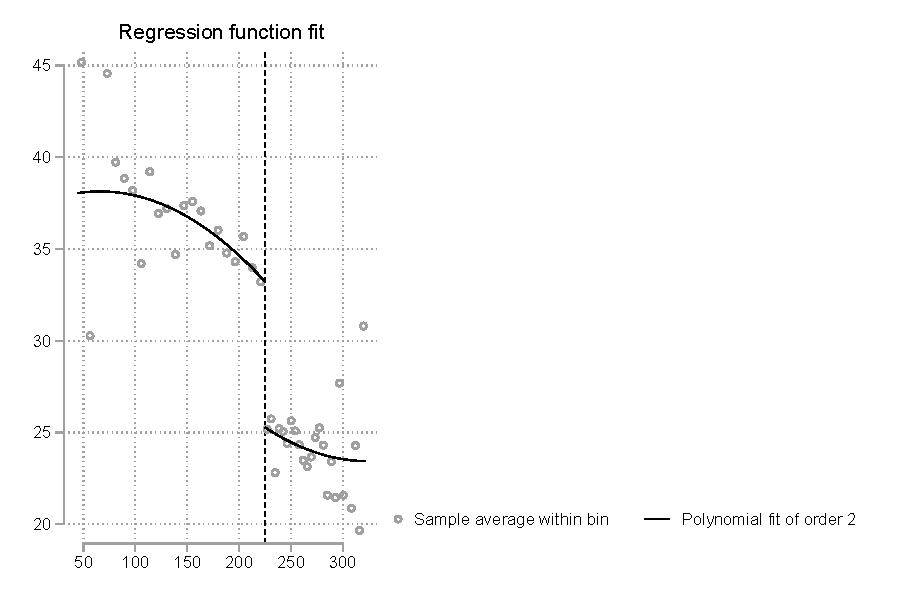
\includegraphics{hw6q2.pdf}
    \caption{MPG(Predicted) vs length}
    \label{fig:my_label}
\end{figure}

\subsection{}
The F test gives a really high score of 38079. This tells us it might be a reasonable instrument. 
\end{document}
